%Copyright 2014 Jean-Philippe Eisenbarth
%This program is free software: you can
%redistribute it and/or modify it under the terms of the GNU General Public
%License as published by the Free Software Foundation, either version 3 of the
%License, or {at your option} any later version.
%This program is distributed in the hope that it will be useful,but WITHOUT ANY
%WARRANTY; without even the implied warranty of MERCHANTABILITY or FITNESS FOR A
%PARTICULAR PURPOSE. See the GNU General Public License for more details.
%You should have received a copy of the GNU General Public License along with
%this program.  If not, see <http://www.gnu.org/licenses/>.

%Based on the code of Yiannis Lazarides
%http://tex.stackexchange.com/questions/42602/software-requirements-specification-with-latex
%http://tex.stackexchange.com/users/963/yiannis-lazarides
%Also based on the template of Karl E. Wiegers
%http://www.se.rit.edu/~emad/teaching/slides/srs_template_sep14.pdf
%http://karlwiegers.com
%\documentclass[letterpaper,10pt]{article}
\documentclass[onecolumn, draftclsnofoot,10pt, compsoc]{IEEEtran}
\usepackage{listings}
\usepackage{underscore}
\usepackage[bookmarks=true]{hyperref}
\usepackage[utf8]{inputenc}
\usepackage[english]{babel}
\usepackage{graphicx}
\usepackage{amssymb}
\usepackage{amsmath}
\usepackage{amsthm}
\usepackage{afterpage}
\usepackage{hyperref}

\usepackage{alltt}
\usepackage{float}
\usepackage{color}
\usepackage{url}
\usepackage{setspace}

\usepackage{enumitem}

\usepackage{geometry}

\usepackage{titling}
\usepackage{rotating}
\usepackage{pgfgantt}
\usepackage{graphicx}
\usepackage{xcolor}
\usepackage{anyfontsize}
\usepackage{amsmath}
\usepackage[linesnumbered,ruled]{algorithm2e}
\ganttset{group/.append style={orange},
milestone/.append style={red},
progress label node anchor/.append style={text=red}}

\newcommand\blankpage{
    \null
    \thispagestyle{empty}
    \addtocounter{page}{0}
    \newpage}

\geometry{textheight=9.5in, textwidth=7in}
\hypersetup{
    bookmarks=false,    % show bookmarks bar?
    pdftitle={Software Requirement Specification},    % title
    pdfauthor={Jean-Philippe Eisenbarth},                     % author
    pdfsubject={TeX and LaTeX},                        % subject of the document
    pdfkeywords={TeX, LaTeX, graphics, images}, % list of keywords
    colorlinks=true,       % false: boxed links; true: colored links
    linkcolor=blue,       % color of internal links
    citecolor=black,       % color of links to bibliography
    filecolor=black,        % color of file links
    urlcolor=purple,        % color of external links
    linktoc=page            % only page is linked
}%

% 1. Fill in these details
\def \CapstoneTeamName{		Deep Learning on Embedded Platform}
\def \CapstoneTeamNumber{		14}
\def \GroupMemberOne{			Christopher Johnson}
\def \GroupMemberTwo{			Gabe Morey}
\def \GroupMemberThree{			Luay Alshawi}
\def \CapstoneProjectName{		AI Gaming}
\def \CapstoneSponsorCompany{	NVIDIA}
\def \CapstoneSponsorPerson{		Mark Ebersole}

\def \DocType{	%Problem Statement
				%Requirements Document
				%Technology Review
				Design Document
				%Progress Report
				}

\newcommand{\NameSigPair}[1]{\par
\makebox[2.75in][r]{#1} \hfil 	\makebox[3.25in]{\makebox[2.25in]{\hrulefill} \hfill		\makebox[.75in]{\hrulefill}}
\par\vspace{-12pt} \textit{\tiny\noindent
\makebox[2.75in]{} \hfil		\makebox[3.25in]{\makebox[2.25in][r]{Signature} \hfill	\makebox[.75in][r]{Date}}}}

\begin{document}
\begin{titlepage}
    \pagenumbering{gobble}
    \begin{singlespace}
    	%
\includegraphics[height=4cm]{coe_v_spot1}
        \hfill
        % 4. If you have a logo, use this includegraphics command to put it on the coversheet.
        %\includegraphics[height=4cm]{CompanyLogo}
        \par\vspace{.2in}
        \centering
        \scshape{
            \huge CS Capstone \DocType \par
            {\large\today}\par
            \vspace{.5in}
            \textbf{\Huge\CapstoneProjectName}\par
            \vfill
            {\large Prepared for}\par
            \Huge \CapstoneSponsorCompany\par
            \vspace{5pt}
            {\Large\NameSigPair{\CapstoneSponsorPerson}\par}
            {\large Prepared by }\par
            Group\CapstoneTeamNumber\par
            % 5. comment out the line below this one if you do not wish to name your team
            \CapstoneTeamName\par
            \vspace{5pt}
            {\Large
                \NameSigPair{\GroupMemberOne}\par
                \NameSigPair{\GroupMemberTwo}\par
                \NameSigPair{\GroupMemberThree}\par
            }
            \vspace{20pt}
        }
        \begin{abstract}
        	In this document we describe the design of a deep learning system developed to learn how to play the arcade game Galaga.
		Galaga is an arcade shooter which was released in 1981 by Namco [1].
		This system is designed with the ultimate goal of being turned into a course for the NVIDIA Deep Learning Institute.
		The documentation will outline exactly what hardware will used, how the system will be put together, and what methods will be used in a way that allows others to recreate this project.
        \end{abstract}
    \end{singlespace}
\end{titlepage}

\newpage
\pagenumbering{arabic}
\tableofcontents

\section{Overview}

\subsection{Purpose}

The main aim of this document is to give others a thorough enough understanding of the project and its design to replicate the project.
The reader of this document should walk away able to understand how the system works and why it was designed this way.
The document must be thorough enough for NVIDIA to recreate the project and package the design into a training course on deep learning.
\newline
\newline
This project is to be used to produce a training course for NVIDIA's Deep Learning Institute.
After the project is complete it will be handed off to NVIDIA for the purposes of accomplishing this goal.
To that end the documentation has been designed to provide readers a clear path towards building this system themselves.

\subsection{Scope}

This document outlines the design of a system for teaching a deep learning neural network how to play the game Galaga.
The sections of this document will outline the system details, setup, and all things necessary to understand how and why the project is designed.
Hardware required, API's to be used, and setup will be detailed as part of the project design.

\subsection{Context}

This system is not designed for an average computer user.
This system is a showcase of possibilities when working with Neural Networks.
As such, no real UI will be developed for the purposes of this project.
Average people may see the result of the final project by viewing the network play Galaga.
\newline
\newline
This system is designed for developers.
Developers should be able to do a project like this as an introduction to deep learning neural networks.
The documentation provided here reflects this focus and is written with developers in mind.

\subsection{Summary}

The neural network created for this project will be able to play Galaga.
Its design is based on GoogLeNet, a convolutional neural network designed in coordination with Google Inc.,  University of North Carolina, Chapel Hill, University of Michigan, and Magic Leap Inc. [2].
This neural network will undergo two main phases of training.
One training phase will be done with just still images, while the second will involve live image feed from the game Galaga.
The system will run inference on the Jetson TX1 developer kit, which will interface between a seperate computer via a controller.
The Jetson will be wired to the controller to control the game on the seperate computer.
Cloud computing GPUs will be used to handle the training.
In total, the system should be able to learn how to play Galaga, and then continually improve as it plays.

\subsection{References}

[1] F. Rojas, "Galaga (Namco)," in gaminghistory101.com, Gaming History 101, 2012. [Online]. Available: https://gaminghistory101.com/2012/03/22/galaga/.\newline
[2] C. Szegedy et al., "Going Deeper with Convolutions," in cs.unc.edu. [Online]. Available: https://www.cs.unc.edu/~wliu/papers/GoogLeNet.pdf.\newline

\subsection{Definitions}
\begin{description}

  \item[Neural Network:] A multilayered graph structure containing nodes, referred to as neurons, and weights that affect how likely the node is to be chosen when confronted with a decision.
The weights of nodes are decided through training the network, and a traversal of the graph acts as a large chain of decisions as the neural network is confronted with situations.

  \item[Deep Learning:]  Using a layered neural network constructed by GPU processing to teach a computer how to accomplish a specific task.

  \item[Convolutional Neural Network:] A neural network specifically designed to take images as input.
It uses convolutional layers to process the image into a more manageable chunk of data and extracts the information relevant to the network.

  \item[Caffe:] A code framework that allows for complex mathematical operations that are required for training a neural network.

  \item[API:] Application Programming Interface

  \item[Jetson TX1:] Quad core embedded system designed for power efficiency and deep learning projects

  \item[OS:] Operating system

  \item[OpenCV:] (Open Source Computer Vision) is a library that can be used with different languages(C, C++, Java, Python, etc.). It provides standard functionalities such as image capture, Faces recognition, Gesture recognition, Motion tracking, Mobile robotics, Object identification and Image manipulation.

  \item[Galaga:] Galaga is an arcade video game released in 1981 by Namco [1]. The player takes control of a small space ship and must shoot at and dodge waves of alien space ships.
Victory in a level is achieved by destroying all enemy ships.

\end{description}

\section{Design}

\subsection{Introduction}

This section lays out several viewpoints from which we have approached the design of this project.
Each component will be matched under an appropriate viewpoint that gives the reader a clear idea of how the design was apparoached.
Each subsection details a different set of components, many of which will be lumped together, which constitute a major piece of the final design.
There are three main viewpoints from which we have approached the design:
\begin{itemize}
  \item Structure Viewpoint: Design elements approached from a structural level.

  \item Information Viewpoint: Design elements approached from a perspective of data flow operations and data processing.

  \item Interaction Viewpoint: Design elements relevant to getting systems to integrate with each other. Particularly focused on hardware setups required for the rest of the process.
\end{itemize}

Each viewpoint is covered in more depth in its respective section.

\subsection{Structure viewpoint}%Gabe

This section covers integral structural elements of the system and how they come together.
Tools used will be covered to give readers an idea of how we set up the system structure.
The heart of this structure is our neural network set-up.

\subsubsection{Neural network setup}%Gabe

The neural network set-up itself is a multi-layered combination of components.
At the basic level of design, our neural network follows the architecture known as GoogLeNet.
GoogLeNet is designed, as a convolutional neural network, specifically to process images and categorize them.
At the architectural level it has 22 layers, each consisting of special modules [2].
These modules have a structure similar to that outlined in figure \ref{fig:4.1}.
\newline
\newline
\begin{figure}
  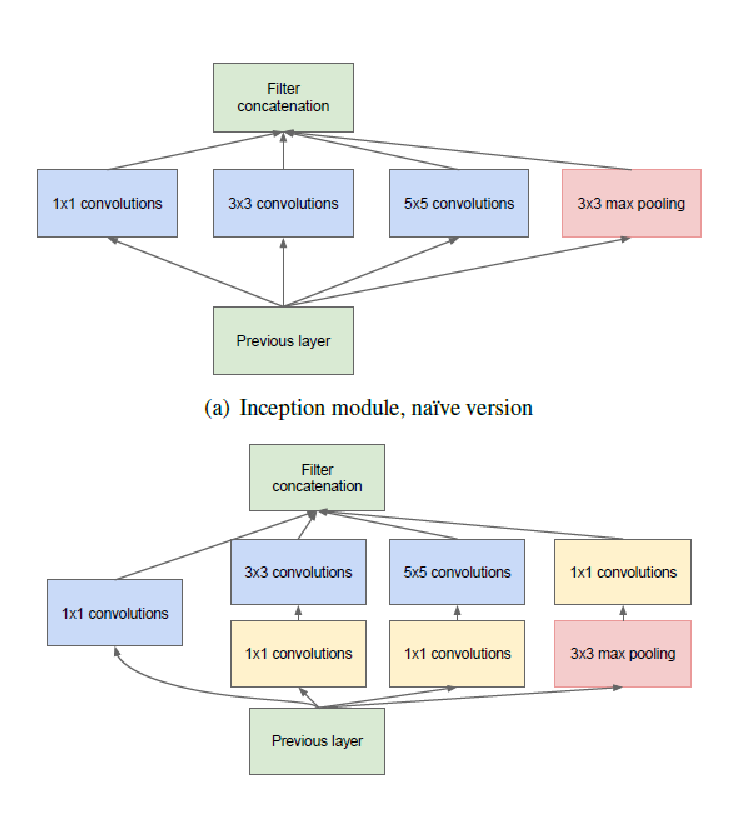
\includegraphics{GoogLeNetModule.eps}
  \caption{GoogLeNet Module}
  \label{fig:4.1}
\end{figure}The network set-up provided by GoogLeNet needs to be accessed with a framework, as well as modified slightly for this project's needs.
For the framework this project uses Caffe.
Caffe allows for command line instructions to be sent to define the network.
To set up the network and Caffe properly we are using a program called DIGITS.
DIGITS is a neural network set-up application designed and released by NVIDIA.
It gives an easy interface for setting up the exact parameters for learning as well as building the network up.
The exact parameters we need for the set-up of this net are unknown at this time and will be added when available.
\newline
\newline
Training of the neural network will be done on NVIDIA GPUs on the Amazon Web Services cloud.
The network will run its calculations on the cloud and send its response down to the Jetson TX1.
There the response will be interpreted into the proper action.
\newline
\newline
The structural goal of the neural net changes between two stages.
In the first stage, the structure of the neural net is meant purely to teach it how to recognize and categorize in game objects from images.
In the second stage, the neural network will be deployed on the Jetson TX1 and will take active game information.
It will use that information to make one of three choices: move left, move right, or shoot.
More detail on the training will be given in section \ref{sssec:num2}.

\section{Information viewpoint}\label{sssec:num2}%Luay

The data in this section consists of image processing of the game being played as well as the data of the trained neural network.
This section will go in depth of both how image processing will be done as well as different ways to train and improve the neural network.
A pseudocode will be included to give an overview of where these data will be used in this project.
Also, the pseudocode in \ref{sssec:num3} will include a general algorithm of how the Jetson will be able to play the game Galaga using the image capture data and the neural network.

\subsection{Set up image dataset}%Luay

OpenCV is a useful tool for this deep learning project.
It will be used as a helper tool to prepare the images for each object in the game such as players, enemies, and bullets.
A script will be written in python which will use OpenCV to crop, resize, and filter the game images when needed.
The goal is to have a full set of the game images and their labels which will be used to train the neural network.
Using OpenCV at this phase is optional, but, due to the need of fast image manipulation, OpenCV can be used to do this task easily and will help to save time and effort.
Although, collecting objects’ images can be done manually, eventually, OpenCV will be used to resize the collected images to a consistent size.

\subsection{Image processing}%Luay

After having a trained neural network, a software written in python will start by loading the necessary dependencies, which are OpenCV, Caffe, and the trained neural network.
At this step, it’s important to convert the given neural network to an object that OpenCV can understand.
Then, a video capture of the game will take a place to record the monitor where the game is being played using OpenCV's API
The hardware connection of the camera as well as the control mechanism of the game shall be explained in section \ref{sssec:num1}.
Since videos are just consecutive images, OpenCV will be used to process the images by comparing them with the trained neural network.
The idea is to identify the location of each dangerous object that could reduce the player's life so the Jetson TX1 can send a command to the game controller and move the player away from the harmful object.



\subsection{Neural training methods}%Gabe

The training of the neural network will be done in two stages.
In the first stage, we will be using images created from the game to teach the network how to recognize in game objects.
Given that GoogLeNet was designed with image categorization in mind, this set-up will be easy to create and bring to functionality.
We will feed the network with images doctored by OpenCV and it will interpret them and label them.
Once it has a high degree of success in correctly identifying in game objects, we will take the training to stage two.
\newline
\newline
In the second stage of training we will be feeding the network images directly from live game progress.
The game will be running and the network will be deployed on the Jetson.
The network will be given the ability to take actions based on the objects it identifies on screen.
Positive feedback will be given to the neural network when it correctly kills an enemy or completes a level.
Negative feedback will be given to the network when it dies, gets a game over, or loops too long doing nothing.
As the neural network plays the game, it will improve performance and eventually be considered proficient.

\subsection{Data visualization}%Chris

It was necessary to figure out how to display the results of each round.
We decided it would be best to have a summary, graphical display of the data at the end of the playthrough.
Once the program runs out of lives, a screen will appear, graphing statistics about the machine's performance.
These statistics will include things such as how long the machine lasted, how many levels it completed, which enemies or objects took away the most lives, and so on.
Having detailed and easily readable data is key to knowing how to train the machine to keep performing better in the game.


\newpage

\subsection{Pseudocode}\label{sssec:num3}%Chris
\begin{algorithm}
  % Load necessary packages for openCV, and Caffe.\.
  % Load the trained net.\.
  % Convert the trained net to an object which OpenCV understands.
  % Start video capture.
  % For each frame in the video capture:
  \emph{Load necessary packages for openCV, and Caffe}\;
  \emph{Load the trained net}\;
  \emph{Convert the trained net to an object which OpenCV understands}\;
  \emph{Start video capture}\;
  \ForEach{frame in the video capture}{
    \If {there is a match in the frame of an enemy object from the trained neural network}
    {
      \nl$enemy_x,enemy_y\leftarrow Coordinates Of Enemy Object$\;
      \emph{move the player away from the coordinates enemy_x, enemy_y}\

    }

  }

    \caption{Pseudocode}
\end{algorithm}

\section{Interaction Viewpoint}\label{sssec:num1}%Chris

This section details how our physical hardware components interact to form a cohesive system.
It will outline several pieces of hardware used to realize the goal of playing galaga.

\subsection{Hardware setup}%Chris

While working with the Jetson TX1 there are several things that we needed to decide.
These included our methods to communicate with our client, and the hardware used with the Jetson.
Choosing out hardware was key to determining how each piece would fit into the design.
\newline
\newline
Our project will actually need to be able to control the game.
Inputs from the neural net need to be received by the game so that it can be played.
To do this we decided not to use the standard keyboard.
Using a keyboard requires a lot of additional coding to map the Jetson to the controls.
Instead we decided to find a game controller that we will hardwire to the Jetson TX1.
A game controller will significantly reduce the work load because it will already contain a lot of built in functionality that we need to connect it to the Jetson.
The Jetson will be able to control the game using the controller's built in functionality.
This controller will be hooked up to another computer that will actually be running the game.
\newline
\newline
\begin{figure}
  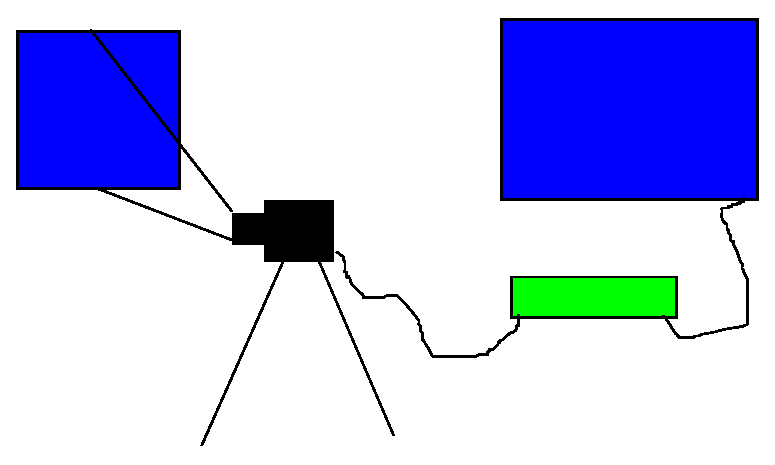
\includegraphics[width=\textwidth]{design.eps}
  \caption{Hardware Layout}
  \label{fig:4.2}
\end{figure}% Figure \ref{fig:4.3} shows the basic layout.
Since the Jetson has to learn how to play the game on its own it needs to be able to see the game.
For this we decided to use the camera sent to us by our client.
This was the simplest option seeing as we can connect the camera directly to the Jetson.
The camera will be connected to the Jetson and aimed at the monitor, which is connected to the computer running the game.
The program will first be trained by being given the video input to recognize and characterize objects within the game.
We will set up tables so that the neural net will be able to store information such as the locations of objects.
Once the objects and tables are set up the neural net will be able to train itself by playing the game using the controller.
Its decisions will be based on the table of information that it stores and will increasingly be able to survive the game longer.
Eventually the neural net will learn to respond to certain patterns in the table in order to become better at the game.

\section{Conclusion}
The goal of this design document is to provide the how to of this deep learning project which will be turned to the NVIDIA's deep learning institute to use it in a deep learning course.
The overall steps for this document are to teach the Jetson TX1 to play the game Galaga by training a neural network to identify game objects and become effectively able to move the player away from enemies.
This can be done based on three major phases which are preparing images for the game objects, training a neural network based on the set of images with labels, and finally by using a camera connected to the Jetson TX1 while the game hosted on a different machine that is being controlled using the Jetson TX1 and a controller input.

\end{document}
